\chapter{Minimal models}\label{chap1}%chap 1

\markright{\thechapter. Minimal models}

\textbf{Summary of results.}\pageoriginale The subject of these lectures is the
theory of birational transformations of two dimensional algebraic
varieties, or more generally two dimensional reduced schemes over a
base, scheme. We first recall the definition of a birational map. Let
$X$ and $Y$ be two preschemes over a base scheme $B$ and $f$ and $g$
$B$-morphisms of open dense sets $U$ and $V$ respectively of $X$ into
$Y$. We shall say that $f$ and $g$ are equivalent if they coincide, as
morphisms of $B$- preschemes, on an open dense subset $W$ of $U \cap
V$. This is clearly  an equivalence relation, and equivalence classes
are called  $B$-\textit{rational maps} (or \textit{rational maps over
  $B$}) of $X/B$ into $Y/B$. A rational map of $X/B$ into $Y/B$ is
called \textit{birational} if it admits a representative which is a
$B$-isomorphism of an open dense subset of $X$ on to an open dense
subset of $Y$, and $X$ and $Y$ are then said to be birationally
equivalent over $B$. 

For obvious reasons, it is in general not possible to `compose' two
rational maps, and consequently, we cannot from a category whose
morphisms are rational maps. However, if $X$ and  $Y$ are irreducible
$B$-pre\-schems and $\varphi$ a rational map of $X/B$  into $Y/B$ such
that the image of some representative of $\varphi$ is dense in $Y$ and
$\psi$ a rational map of $Y/B$ into a third $B$-prescheme $Z/B$, it is
possible to define uniquely the `composite map' $\psi \circ \varphi$.
Thus,\pageoriginale when $X$ and $Y$ are irreducible, a rational map
$\varphi$ of $X/B$ 
into $Y/B$ birational if and only if there is a rational map $\psi$ of
$Y/B$ into $X/B$ such that $\psi \circ \varphi$ is defined and is the
identity map of $X/B$ (that is, contains the identity morphism of
$X/B$ as a member) and $\varphi \circ \psi$ is the identity map of $Y/B$.   

We are mainly interested in the case when the base scheme $B$ is a
noetherian integral scheme of dimension $\leq 1$ which is regular. We
recall that a prescheme is \textit{regular} if the rings of its points
are regular. (For the definitions of the other terms used, see $\EGA$,
I). Thus $B$ can be either $(a) B = \Spec k$, $k$ a field, or $(b)$
an irreducible noetherian scheme such that for every close point $ b
\in B$, the local ring $\mathscr{O}_b$ is a discrete (rank 1)
valuation ring. 

First consider the case when $X$ is an irreducible and reduced
$B$-scheme of finite type and of dimension $1$. Let $R(B)$ and $R(X)$
denote the fields of rational functions (that is rational maps into
Spec $\mathbb{Z} [T]$) of $B$ and $X$ respectively. When we are in
the case $(a)$ where $B$-Spec $k$, it is well-known [$\EGA$ II, 7.4]
that there is an irreducible, regular, proper (and even projective)
$k$-scheme $X'$ and a birational map $\varphi$ of $X'$ into $X$ over
$k$. Further, if $\psi$ is a rational map of $X$ into a $k$-proper
scheme $Y/k$, $\psi \circ \varphi$ extends to (or has as a representative)
a \textit{morphism} of $X'$ into $Y$ over $k$. [$\EGA$ II, 7.4]: In
particular, if $X$ is itself $k$-proper, $\varphi$ is a morphism of $X'$
into $X$. It follows that $X'$ is uniquely determined upto a
$k$-isomorphism, by the conditions that it be regular, $k$- proper and
birational\pageoriginale with $X$. The local rings of the closed
points of $X'$ can 
be canonically identified with the discrete valuation rings in $R(X)$
containing $k$ and having $R(X)$ for quotient field. When we are in
case $(b)$, it can happen that the image of $X$ under the structural
morphism is a single point $b_o$ of $B$. In this case, since $X$ is
reduced, we can factor this morphism as $X \rightarrow \Spec k(b_o)
\rightarrow B$ where $k(b_o)$ is the field of residues at $b_o$ and
the second morphism is the canonical morphism of Spec $k (b_o)$ into
$B$. Thus we are essentially in case $(a)$. However, if the image of
$X$ in $B$ does not reduce to a single point, since $X$ is irreducible
and $B$ is one-dimensional, the image of $X$ must be dense in $B$. By
composition therefore, we get a monomorphism of $R(B)$ into $R(X)$,
and $R(X)$ may be considered as a finite algebraic extension of
$R(B)$. Let us assume that for any affine open subset $B'$ of $B$, the
integral closure of its ring $\Gamma (B',\mathscr{O}_B)$ (considered as a
subring of $R(B)$) in the field $R(X)$ is a finite $\Gamma (B',
\mathscr{O}_B)$-module. (This is a mild assumption, and is fulfilled, for
example, if $R(X)$ is separable over $R(B)$ or if $B$ is an algebraic
scheme). Let $X'$ be the normalisation of $B$ in the field $R$
 is an field $R(X)$ (EGA, II, 6.3). Then $X'$ is irreducible, regular,
 and proper over 
$B$ and there is a birational map $\varphi$ of $X'/B$ into $X/B$. As
in the earlier case, for any rational map $\psi$ of $X/B$ into a scheme
$Y$ proper $B$, $\psi \circ \varphi$ extends to a $B$-morphism of $X'$ into
$Y$, $\varphi$ is itself a morphism if $X/B$ is proper, and $X'$ is
uniquely determined upto a $B$-isomorphism by the conditions
that\pageoriginale it be 
irreducible, regular, $B$-proper and birationally equivalency to
$X/B$. The local rings of closed points of $X'$ are precisely the
discrete valuation rings having $R(X)$ for quotient field and
dominating the local ring of some closed point of $B$. 

Thus, when $\dim X=1$ (and $X$ and $B$ satisfy the conditions  above),
the picture is very simple. Among the $B$-schemes birationally equivalent
to $X/B$, there is a unique one (upto a $B$-isomorphism)- $X'/B$ which is
regular and $B$-proper. If further $X/B$ is proper, we have a birational
morphism $X' \rightarrow X$ over $B$. The local rings of closed points
of $X'$ are discrete valuation rings with quotient field $R(X)$
which dominate the local ring of some closed point of $B$. 

The situation is far from being this simple, even when dim $X=2$, as
is shown by the following two examples. We use the usual language of
algebraic varieties. 

\begin{exam}\label{chap1:exam1}%exam 1.
  Let $X = \mathbb{P}^2 (k)$ be the two dimensional projective space
  over $k$  with homogeneous co-ordinates $(x_0, x_1, x_2)$. Then $X$
  is regular and $k$-proper. Consider the rational map $(x) \rightarrow
  (y)$ of $X$. into itself determined by the equations 
  $$
  y_0 = x_1 x_2, \; y_1 = x_0 x_2, \; y_2 = x_0 x_1
  $$
  and defined on the open subset of $X$ which is the complement of the
  three points $(1,0,0)$, $(0,1,0)$ and $(0,0,1)$. One verifies by
  substitution that the square of this rational map is the identity
  map of $X$ onto itself, so that in particular, this map is
  birational. 

It is\pageoriginale in fact a biregular isomorphism of the complement
of the lines $x_0 = 0$, $x_1 = 0$ and $x_2 = 0$ onto itself. But the
entire line $x_0 = 0$ is mapped onto the single point $(1,0,0)$ and
similarly the lines $x_1 = 0$ and $x_2 = 0$ are mapped onto the points
$(0,1,0)$ and $(0,0,1)$ respectively. Thus, this rational map cannot
extend to an automorphism of $X$.   
\end{exam}

\begin{exam}\label{chap1:exam2}%exam 2.
  Assume $k$ algebraically closed, and Let $\mathbb{F}^2$ be a
  non - degenerate quadratic surface in $\mathbb{P}^3$. Then
  $\mathbb{F}^2$ is regular and $k$-proper. 

  \begin{figure}[H]
    \centerline{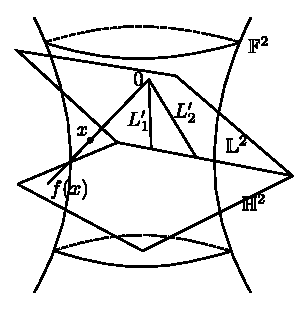
\includegraphics{vol37-figures/fig37-1.eps}}
  \end{figure}
  
  We set up a birational
  correspondence between $\mathbb{F}^2$ and the projective plane
  $\mathbb{P}^2$ by  a method familiar under the name of stereographic
  projection in function theory. Let $0$ be any (closed) point on
  $\mathbb{F}^2$ and $\mathbb{H}^2$ a plane in $\mathbb{P}^3$ not
  containing $0$. For any point $x \in \mathbb{F}^2-\{ 0 \}$, define
  $f(x)$ to be the point of $\mathbb{H}^2$ where the line $0 x$ meets
  $\mathbb{H}^2$. (fig. 1) $f$ is then a morphism of $\mathbb{F}^2 -
  \{ 0 \}$ into $\mathbb{H}^2$. 
\end{exam}

$f$ cannot be extended  to a morphism of $\mathbb{F}^2$ into
$\mathbb{H}^2$, as is shown by a simple calculation. $(f(x)$ tends to
different limits as $x$ approaches $0$ from different directions in
$\mathbb{F}^2$, when $k$ is the filed $\mathbb{C}$ of complex
numbers). Let $\mathbb{L}^2$  be the tangent plane to $\mathbb{F}^2$
at 0, so that\pageoriginale $\mathbb{L}^2$ intersects $\mathbb{F}^2$
along two straight lines $\mathbb{L}^{'}_1$ and $\mathbb{L}'_2$ of
$\mathbb{F}^2$. Then $f$ maps $\mathbb{L}^{'}_i$ onto the points
$\mathbb{L}_i \cap \mathbb{H}^2$, and $f$ is an isomorphism of the
open subset$\mathbb{F}^2 -(\mathbb{L}^{'}_1 \cup \mathbb{L}^{'}_2)$
of $\mathbb{F}^2$ onto the open subset $\mathbb{H}^2 -(\mathbb{H}^2
\cap \mathbb{L}^2)$ of $\mathbb{H}^2$. In particular, $f$ gives a
birational equivalence of $\mathbb{F}^2$ and $\mathbb{H}^2 \simeq
\mathbb{P}^2$. 
 
 In this example not only is $f$ not biregular, but there is
 \textit{no} biregular isomorphism of $\mathbb{F}^2$ and
 $\mathbb{P}^2$. When $k = \mathbb{C}$, this follows from
 the fact that the second Betti-number of $\mathbb{P}^2$ is 1, while
 that of $\mathbb{F}^2$ is 2.  
 
 Our chief concern in these lectures is with the case when dim
 $X=2$. \textit{For this preliminary discussion, we assume for the
   sake of simplicity that $B =$ Spec $k$ where $k$ is algebraically
   closed.} We assume that $X$ is regular and $k$-proper. With the one
 dimensional case in mind, we may ask if we can pick out from among
 the $k$-schemes which are proper over $k$ and birationally equivalent
 to $X$ a unique `model' which has some `nice' properties. The above
 examples show that, unlike the one dimensional case, being regular,
 $k$-proper and birational with $X$ does not ensure uniqueness. Again in
 analogy with the one dimensional case, we may look for an $X'$ which
 is maximal in the birationality class of $X$, in the sense that if
 $Y$ is any other irreducible $k$-proper scheme birationally equivalent
 to $X$ and $ Y \overset{f}{\rightarrow} X'$ is a birational $k$-
 morphism, $f$ is an isomorphism. However, such a maximal model does
 not exits, because of a process of construction, known as dilatation
 or `blowing up a point'. We shall prove its existence later, but we
 shall now describe its essential features.\pageoriginale 
 
 Let $X$ be an irreducible 2 dimensional regular algebraic
 $k$-scheme, and $x$ a closed point of $X$. The dilatation of $X$ at
 $x$ is then an irreducible regular $k$-scheme $Y$ together with a
 proper morphism $f:Y \rightarrow X $ which is birational, $f$ induces
 an isomorphism of $Y-f^{-1}(x)$ into $X - \{ x \}$. The fibre
 $f^{-1}(x)$ is an irreducible curve $C$ in $Y$. These properties
 suffice to fix $Y$ uniquely (upto an $X$-isomorphism) in terms of $X$
 and $x$. One can deduce that $C$ must be isomorphic with the
 projective line $\mathbb{P}'$. Let $D$ be a  regular curve on  $X$
 through $x$. The inverse of $f$ on $X -\{x\}$, defines by restriction
 a morphism $g$  of $D-\{ x \}$ into  $Y$, and since $Y$ is $X$-proper
 and $D$ is  regular at $x, g$ extends to a morphism of $D$ into
 $Y$. (In the case when $k$ is the complex field $\mathbb{C}$, $g(x)$
 must be the limit of $g(y)$ as $y$ tends to $x$ from $D - \{x\}$). It
 can be shown that $g(x)$ depends only on the tangent line to $D$ at
 $x$. Thus to every `direction' at $x$ (that is, a one-dimensional
 subspace of the tangent space to $X$ at $x$), we obtain a point of
 the fibre $f^{-1}(x) = C$. This correspondence can be shown to be
 bijective, and since the set of directions at $x$ can be identified
 with $\mathbb{P}'$, we have a further heuristic confirmation of
 the fact that $C \simeq \mathbb{P}'$,  
  
 The possibility of building such a dilatation associated to any
 regular algebraic $k$-scheme and any closed on it shows that we
 cannot find a ``maximal model'' in the birationality  class of $X$, in
 the sense described in the previous paragraph. And for the same
 reason, we see\pageoriginale that there is no model whose local whose
 rings at closed points are all the regular local rings of dimension 2 of the
 field $R(X)$ containing $k$ and having $R(X)$ for quotient field. One
 might ask if it is not possible to form some of projective limit of
 all regular $k$-proper models of $R(X)$, the maps of this projective
 system being the birational morphisms. This could be done, and has
 also proved to be useful (\cf \cite{key26} \S 17 and \cite{key17}), but
 unfortunately the resulting set does not carry a structure of scheme. 
 
 Is this process of dilatation reversible? In other words, given $Y$
 irreducible, two dimensional, regular, and $k$-proper, and an
 irreducible curve $C$ on $Y$, does there exist an $X$ and a point $x
 \in X$ such that $Y$ is obtained by dilating (or blowing up) $x$ on
 $X$ and $C$ is the fibre $f^{-1} (x)?$ If this is possible, we also
 say that $C$ on $Y$ can be contracted or blown down to a
 point. Clearly, a  necessary condition is that $C$ be isomorphic to
 $\mathbb{P}'$,  Further, let $U$ be an affine open neighbourhood of
 $x$ on $X$, and $V$ the inverse image of $U$ in $Y$.  If $C'$ is any
 irreducible closed curve on $Y$ contained in $V$, the image of $C'$
 in $X$ is proper, affine and irreducible, and hence must be a
 point. Since the morphism is one- one on $Y-C, C'$ must coincide with
 $C$. Thus, any irreducible closed  curve on $Y$ which is
 `sufficiently near' to $C$ must coincide with $C$. This shows
 that such curves on any surface are quite exceptional, and we see for
 instance that on a complete homogeneous surface of any  algebraic
 group, no curve can be contracted to a point. A more precise\pageoriginale
 criterion for the contractibility of $C$ on $Y$ is given  by  a
 theorem  of Castelnuovo, which states that under the above
 assumptions on $Y$ and $C, ~ C$ is contractible to a point if and
 only if $C$ is isomorphic to $\mathbb{P}'$ and the intersection
 number  $(C)$. $(C)$ is $-1$.  
 
 These considerations suggest that given $X/k$ which is regular,
 proper and two dimensional, we should look for an $X'$. having the
 same properties, birationally equivalent to $X$ and \textit{minimal}
 for these properties, in the sense that any birational
 \textit{morphism} $X' \rightarrow Y$, where $Y$ is again regular and
 $k$-proper, is an  isomorphism. An $X'$ satisfying the above
 properties is called a \textit{relatively minimal model} in the
 birationality class of $X$ or for the function  field $R(X)/k$. If
 such a relatively minimal model for $R(X)/k$ is unique upto  a
 $k$-isomorphism, it is called a \textit{minimal} model.  
 
 We are now in a position to be able to state the principal theorems
 that we shall prove. 
 
 We shall show that there always exist relatively minimal models (for
 given $X/k$ or equivalently,) given extension $K/k$  of finite type
 and transcendence degree two.) But these are not always unique, as
 shown by example \ref{chap1:exam2} above. (Both $\mathbb{P}^2$ and
 $\mathbb{F}^2$ 
 are homogeneous spaces, and homogeneous surfaces can be shown to be
 relatively minimal). However, it was discovered by Enriques that this
 is one of a very few examples in which uniqueness fails to hold. He
 found that if all relatively minimal models models are not
 isomorphic, or in other word, if a minimal model fails to exist, $X$
 must be birationally equivalent to a\pageoriginale product  $C \times
 \mathbb{P}'$ where 
 $C$ is a complete curve over $k$. In this case, the relatively
 minimal models are precisely the algebraic fibre spaces over $C$ with
 the projective line $\mathbb{P}'$ as fibre. These are the so called
 ruled surfaces. (We mention that when $C = \mathbb{P}'$, there is
 one exceptional $\mathbb{P}'$ bundle on $C$ which is not relatively
 minimal, but there is a line on this bundle can which be contracted,
 and we obtain the projective plane $\mathbb{P}^2$ which is relatively
 minimal). The above theorem of Enriques is our second principal
 theorem.  
 
 Our first principal theorem says that any birational transformation
 of two dimensional, irreducible, regular and proper $k$-schemes can be
 decomposed into birational transformations of the simplest kind namely
 dilatations. More  precisely, it states that given two irreducible
 regular proper surfaces $X, Y$ over $k$ and a birational
 transformations of $X$ into $Y$, there exists a $Z$ having the
 same properties  and birational \textit{morphisms} $Z
 \overset{f}{\rightarrow} X$ and $Z \overset{g}{\rightarrow} Y$  such
 that (i) $g \circ f^{-1}$  is the given birational equivalence of
 $X$ and  $Y,(ii)$ $f$ and $g$ can respectively be factored as  
 \begin{multline*}
 Z = X_n \overset{f_{n-1}}{\rightarrow} X_{n-1} \rightarrow \dots
 \overset{f_o}{\rightarrow} X_o = X, Z = Y_m
 \overset{g_{m-1}}{\rightarrow} Y_{m-1} \rightarrow \dots \\
 \dots \overset{g_o}{\rightarrow} Y_o = Y, f = f_o o f_1 o\ldots o
 f_{m-1},  g = g o \ldots o g_{m-1}  
 \end{multline*}
 where each $f_i: X_i\rightarrow X_{i-1}$ and $g_j: Y_j \rightarrow
 Y_{j-1}$ is a dilatation. 

Analogues of these theorems also hold in the `arithmetical case'
where $B$ is of dimension 1 (case $(b)$ above). We mention,
however,\pageoriginale that whereas the problem of classifying ruled
surfaces over a 
curve $C$ (or equivalently, the classification of vector bundles of
rank two on $C$) has been treated by many authors, the analogous
problem of classifying the relatively minimal models over space
$\mathbb{Z}$ for example, has not been considered. 

Our principal tool will be the intersection theory of divisors on a
two-dimensional scheme. However, we meet here a difficulty. Namely, in
the case of a regular surface $X$, we can define an intersection
number. $(C_1. C_2)$ of two divisors in such a way that $(C.(f)) = 0$ if
$f$ is a function, only of $X$ is complete. If $X$ is a scheme of
dimension 2, proper over Spec $\mathscr{O}$, where $\mathscr{O}$ is
a Dedekind domain, the situation is different because spec
$\mathscr{O}$ itself is not, in any sense, complete. 

Fortunately, the fibres of $X \rightarrow \Spec \mathscr{O}$ are
complete and we  can define $(C_1.C_2)$ with good properties when $C_1$
is contained in a fibre and $C_2$ is an arbitrary divisor. This
incomplete intersection theory is sufficient for our purposes. Still
it would be very interesting to find a general definition. This seems
possible in the case where is the ring of integers in a number
field. The intersection function should naturally involve the infinite
primes of $\mathscr{O}$ since these serve to ``compactify'' Spec
$\mathscr{O}$. When the general fibre of $X\rightarrow$ Spec
$\mathscr{O}$ is an elliptic curve, Tate has defined a function that
has all the desired properties of the intersection number and Neron
has proved for this function a product formula which can be considered
as an expression of the global intersection  number as a sum of local
ones (See $S$. Lang ``Les formes  bilineaires de Neron et Tate'',
Seminaire Bourbaki No. 274, 1963/64).  
